\documentclass{article}
\usepackage[pdfcreator={LaTeX}]{hyperref}
\usepackage{graphicx}
\usepackage[utf8]{inputenc} 
\usepackage[ngerman]{babel}

\usepackage[section,toc]{glossaries}\makeglossaries

\newglossaryentry{Regelwerk}{name=Regelwerk,
	plural = Regelwerke,
	description={Regeln eines bestimmten Kartenspiels}
}
\newglossaryentry{Client}{name=Client,
	plural = Clients,
	description={Ein Spieler (bzw. Computer des Spielers) der das Online-Kartenspiel nutzt.}
}
\newglossaryentry{Server}{name = Server,
	description={Rechner, der das Online-Kartenspiel zur Verfügung stellt}
}
\newglossaryentry{Lobby}{name = Lobby,
	description={Ort, an dem Spieler ein Kartenspiel auswählen oder beitreten können}
}
\newglossaryentry{Spielleiter}{name = Spielleiter,
	description={Derjenige, der in der Lobby ein neues Spiel erstellt}
}
\newglossaryentry{Erstellungsfenster}{name = Erstellungsfenster,
	description={Fenster in welchem der Spielleiter das Spiel festlegt.}
}
\newglossaryentry{Wartefenster}{name = Wartefenster,
	description={Fenster auf welchem man sich befindet, während man darauf wartet, 
		dass die Mindestteilemerzahl erfüllt ist und das Spiel gestartet wird. }
}

\begin{document}
\begin{titlepage}

\begin{center}
\textbf{\textsc{\LARGE Pflichtenheft}}

{\large \today}

\vspace{2cm}
\includegraphics{Bild}

\vspace{2cm}

\begin{tabular}{|c|c|c|}\hline
   Phase & Verantwortlicher & E-Mail \\ \hline\hline
   Pflichtenheft & Alina  Meixl  &  alina@meixl.de \\ \hline
   Entwurf & Viktoria Witka & witkaviktoria@freenet.de \\ \hline
   Spezifikation & Daniel Riedl & dariedl14@yahoo.de \\ \hline
   Implementation & Andreas Altenbuchner& a.andi007@gmail.com\\ \hline
   Verifikation &Patrick Kubin & kubin@fim.uni-passau.de\\ \hline
   Präsentation & w& w\\ \hline
 \end{tabular}

\end{center}

\end{titlepage}


\tableofcontents

\section{Zielbestimmung}
Ein Online-Multiplayer Kartenspiel.

\subsection{Musskriterien}
Es gibt einen \gls{Server} der das Spiel verwaltet und \glspl{Client} die spielen.
\subsubsection{\gls{Server}}
\begin{itemize}
	\item \glspl{Client} können einen Benutzernamen auswählen und sich anschließend mit dem Server verbinden.
		Der Benutzername muss Eindeutig sein, ansonsten wird eine Warnmeldung ausgegeben.
	\item Es gibt eine \gls{Lobby} in der ein Spieler die Möglichkeit hat, Spiele zu erstellen und offenen Spielen beizutreten.
	\item Es gibt einen Chat in der \gls{Lobby}.
	\item Mehrere parallel laufender Spiele auf einem Server werden ünterstützt.
	\item Regelauswertung mit Überprüfung erlaubter Aktionen, Punktezählung und  Kartenausgabe.
	\item Die Spiele Hearts und Wizard sind verfügbar.	
	\item Chat mit Mitspielern während eines Spiels ist möglich.
	\item Schutz vor Cheats (Mehrfachanmeldung?)
\end{itemize}

\subsubsection{\gls{Client}}
\begin{itemize}
	\item GUI
	\begin{itemize}
		\item Darstellungsfenster, das mindestens bei der Auflösung von 1024x768 Bildpunkten benutzt werden kann.
		\item Darstellung des laufenden Spiels. Es wird die eigene Hand offen und die Hände der anderen Spieler verdeckt 					angezeigt. Je nach Spiel gibt es einen allgemeinen Ablagestapel in der Mitte des Spielfeldes oder individuelle 					Ablagestapel vor der Hand des jeweiligen Spielers. Der Zähler für Punktestand, gemachte Stiche, übrige Karten 					etc. befindet sich neben  der Hand des jeweiligen Spielers. Für die Gegenspieler wird zusätzlich der Name über 					der Hand angezeigt.)
		\item Eine Karte wird durch einmaliges Anklicken ausgewählt und durch ein Zweites anklicken abgelegt. Es gibt ein extra 					Fenster um die zu verschiebenden Karten bei Hearts bzw. die Stichansage bei Wizard auszufüren.
		\item Die GUI muss den Benutzer sinnvoll unterstützen und benutzerfreundliche Eingabeelemente anbieten.
		\item Die Darstellung und das Spiel müssen flüssig laufen.
		\item Die GUI darf nicht vom \gls{Regelwerk} abhängen.
		\item Beim Start kann der Spieler einen eindeutigen Benutzernamens auswohlen und die IP des \gls{Server}s angeben
		\item In der \gls{Lobby} werden offene Spiele angezeigt und es gibt die Möglichkeit ein neues Spiel zu erstellen oder 					einem Existierenden beizutreten.
		\item Chat in der \gls{Lobby} und während des Spiels ist möglich
	\end{itemize}
	\item Modell
	\begin{itemize}
		\item Verwaltung der Verbindung mit dem \gls{Server}
		\item Verwaltung des aktuellen Spielzustands (soweit \gls{Client} bekannt)
		\item Vorab-Regelauswertung zur Unterstützung des Nutzers (ungültige Spielaktionen sind nicht durchführbar in der 					GUI)
	\end{itemize}
\end{itemize}

\subsection{Wunschkriterien}
\begin{itemize}
	\item Weitere \glspl{Regelwerk} (Uno, Mau-Mau, Black Jack)
	\item Statistiken, die nach dem Spiel angezeigt werden. Sie zeigen die Plazierung pro Runde.
	\item Mehrere Sprachen werden unterstützt (Deutsch, Englisch, evtl. Bayrisch)
	\item Anpassung der GUI durch Spieler ist möglich (Änderung von Hintergrundbild, Kartenrückseite)
	\item Es gibt die Möglichkeit seinem neu erstellten Spiel einen Namen zu geben
	\item Passwortauswahl um Beitritt zu offenen Spielen einzuschränken ist möglich
	\item Nach jedem Spiel kann entschieden werden, ob eine weitere Runde gestartet werden soll
\end{itemize}

\subsection{Abgrenzungskriterien}
\begin{itemize}
	\item Beitreten eines bereits laufenden Spieles nicht möglich
	\item keine Persistenz der Daten über mehrere Sessions, keine Registrierung
	\item keine KI
	\item Spiel wird nicht fortgesetzt, sobald ein Spieler es verlässt
	\item Es werden nur 3-6 Spieler unterstützt
	\item Es gibt keinen Schimpfwortfilter
\end{itemize}

\section{Produkteinsatz}
\subsection{Anwendungsbereich}
Ein Kartenspiel, welches im Freundeskreis oder mit Fremden über das Intenet gespielt werden kann.
\subsection{Zielgruppe}
Personen, die gemeinsam über ein lokales Netzwerk oder das Internet spielen möchten. 
\subsection{Betriebsbedingungen}
Dauerbetrieb der Software.

\section{Produktumgebung}
\subsection{Software}
	\begin{itemize}
		\item \gls{Client}
		\begin{itemize}
			\item Betriebssystem Microsoft Windows, Mac OS X oder Linux mit aktueller Java Laufzeit.
		\end{itemize}
		\item \gls{Server}
		\begin{itemize}
			\item Betriebssystem Microsoft Windows, Mac OS X oder Linux mit aktueller Java Laufzeit.
		\end{itemize}
	\end{itemize}

\subsection{Hardware}
\begin{itemize}
		\item \gls{Client}
		\begin{itemize}
			\item Internetfähiger Rechner
		\end{itemize}
		\item Server
		\begin{itemize}
			\item Internetfähiger Rechner	
			\item Mindestanforderungen des verwendeten Betriebssystems bezüglich Arbeitsspeicher und Rechenleistung 					      müssen erfüllt sein, können jedoch durch die Anzahl der gehosteten Spieler/Spiele steigen.
		\end{itemize}
	\end{itemize}

\section{Produktfunktionen}
\subsection{Startseite}
\begin{itemize}
	\item /F040/ Auswahl vom gewünschtem \gls{Server} und Namen
	\item /F045/ Weiterleitung zur \gls{Lobby}
	\item /F050W/ Auswahl der Sprache
\end{itemize}

\subsection{\gls{Lobby}}
\begin{itemize}
	\item /F060/ Senden einer Nachricht an andere Spieler über den \gls{Server}
	\item /F070/ Einem Spiel beitreten. (Bei Passwort geschützten Spiel Weiterleitung zur Passwortabfrage ansonsten Weiterleitung zum \gls{Wartefenster})
	\item /F080/ Erstellen eines neuen Spiels (Weiterleitung zum \gls{Erstellungsfenster})
	\item /F90/ Verlassen der \gls{Lobby} (Programmende)
\end{itemize}

\subsection{Erstellungsfenster}
\begin{itemize}
	\item /F120/ Auswahl des \gls{Regelwerk}s
	\item /F122/ Eingabe eines Namen für das zu erstellende Spiel
	\item /F124/ Erstellung abbrechen und \gls{Erstellungsfenster} verlassen (Zurückleitung zur Lobby)
	\item /F126/ Erstellen eines neues Spiels (Weiterleitung zum Wartefenster)
	\item /F128/ Hilfe zum Spiel(Wie?)
	\item /F130W/ Möglichkeit ein Passwort für das Spiel zu setzen
\end{itemize}

\subsection{Passwortabfrage}
\begin{itemize}
	\item /F140/ Eingabe des Passworts.
	\item /F142/ Einem Spiel beitreten mit Zugang zum \gls{Wartefenster}
	\item /F145/ Abbrechen und zur \gls{Lobby} zurückkehren
\end{itemize}

\subsection{Wartefenster}
\begin{itemize}
	\item Spieler
	\begin{itemize}
		\item /F160/ Chat mit anderen Spielern im selben Spiel
		\item /F170/ Zurückleitung zur Lobby
	\end{itemize}
	\item Spielleiter
	
	Besitzt alle Funktionen des Spielers
	\begin{itemize}
		\item /F180/ Spieler entfernen
		\item /F190/ Bei /F190/ Auflösung des Spiels
		\item /F200/ Starten des Spiels (Voraussetzung: Mindestanzahl der Spieler erreicht)
	\end{itemize}
\end{itemize}

\subsection{Spiel}
\begin{itemize}
	\item Alle Spiele
	\begin{itemize}
		\item /F210/ Verlassen des Spiels (Folge: Alle Spieler kehren zur Serverlobby zurück)
		\item /F220/ Nachricht senden an andere Spieler
		\item /F230/ Karte spielen (Voraussetzung: Am Zug und Karte erlaubt zu spielen)
		\item /F240/ Hilfe zum Spiel (Wie?)
	\end{itemize}
	\item Herz
	\begin{itemize}
		\item /F260/ Eingabe der gewünschten Stiche zu Beginn jeder Runde
	\end{itemize}
	\item Wizard
	\begin{itemize}
		\item /F360/ Auswahl der Trumpffarbe zu Beginn einer Runde (Voraussetzung: Aufdecken des Zauberers)
		\item /F370/ Eingabe der gewünschten Stiche zu Beginn jeder Runde
	\end{itemize}
	\item Uno (Wunsch)
	\begin{itemize}
		\item /F380/ Ziehen vom Kartenstapel(Ist glaub ich Leistung da es immer automatisch passiert?)
		\item /F390/ Farbwahl bei gespielter Farbauswahlkarte
	\end{itemize}
\end{itemize}

\section{Produktdaten}

\begin{itemize}
	\item /D010/ \gls{Lobby}daten
	 \begin{itemize}
	 	\item Spielerdaten
	 	\begin{itemize}
	 		\item Spielername(eindeutig)
	 	\end{itemize}
	 	\item Spieledaten
	 	\begin{itemize}
	 		\item Spielenamen(eindeutig)
	 		\item Spieltyp
	 		\item Anzahl an Spielern und maximale Anzahl an Spielern
	 	\end{itemize}
	 \end{itemize}
	 \item /D020/ Erstellungsdaten
	 \begin{itemize}
	 	\item \gls{Spielleiter}(eindeutig)
	 	\item Spielernamen(eindeutig)
	 	\item Spieleranzahl und maximale Spieleranzahl
	 	\item Spieltyp
	 	\item Mindestanzahl an Spielern erreicht
	 \end{itemize}
	 \item /D030/ Spieldaten
	 \begin{itemize}
	 	\item Spielname(eindeutig)
	 	\item Spieltyp
	 	\item Anzahl an Spielern
	 	\item Kartenstapel
	 	\begin{itemize}
	 		\item Anzahl verbliebener Karten
	 		\item Karten
	 		\item Ausgabe von Karten
	 	\end{itemize}
	 	\item Zugreihenfolge
	 	\item Spieler
	 	\begin{itemize}
	 		\item Name(eindeutig)
	 		\item Kartenhand
	 		\begin{itemize}
	 			\item Karten
	 			\item Anzahl
	 			\item Spielbar
	 		\end{itemize}	 
	 	\end{itemize}
	 	\item Punktestand und Siegbedingung
	 \end{itemize}
\end{itemize}

\section{Produktleistungen}
\subsection{\gls{Lobby}}
\begin{itemize}
	\item /L100/ Anzeige von eingeloggten Spielern
	\item /L110/ Anzeige von erstellten Spielen	
	\item /L115/ Anzeige des Chatdialoges		
\end{itemize}

\subsection{Erstellungsfenster}
\begin{itemize}
	\item /L120/ Anzeige eines Spiellogos
	\item /L122/ Anzeige einer kurzen Spielbeschreibung --- !! nicht in der Skizze! trotzdem?
\end{itemize}

\subsection{Wartefenster}
\begin{itemize}
	\item /L150/ Anzeigen des Spieltyps
	\item /L155/ Anzeigen der Mitspieler
	\item /L158/ Anzeige des Chatdialoges
	\item /L160/ Ab Mindestanzahl der Spieler kann der Spielersteller des Spiel starten ???
	\item /L170/ \gls{Wartefenster} wird nur aufgelöst wenn der Spielersteller selbst das Spiel verlässt ???
\end{itemize}

\subsection{Spiel}
\begin{itemize}
	\item /L190/ Anzeige der eigenen Karten
	\item /L192/ Anzeige der verdeckten Karten der Mitspieler
	\item /L194/ Anzeige des Ablagestapels
	\item /L195/ Anzeige des Aufnahmestapels
	\item /L195/ Anzeige der Anzahl der restlichen Karten für jeden Spieler
	\item /L200/ Anzeige von Punktestand
	\item /L250/ Anzeige einer Auswertung nach Beendigung einer Runde oder eines Spiels
	\item /L260/ Anzeige des Chatdialoges

---------------------------
	??????
	\item /L040/ Einhaltung der Spielregeln gewährleisten
	\item /L050/ Fehlermeldungen akkumuliert ausgeben
	\item /L060/ Verwaltung mehrerer parallel laufender Spiele
	\item /L070/ Chat und Spiel sollen flüssig laufen
	\item /L080/ Einfache und hilfreiche Bedienbarkeit
	\item /L090/ Schutz vor Cheats
	\item /L100/ Verhinderung langer Wartezeiten
	\item /L110W/ Mehrsprachigkeit unterstützen
\end{itemize}

\section{Benutzeroberfläche}
\begin{itemize}
	\item Startseite: \\ 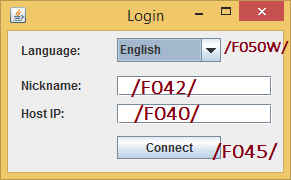
\includegraphics{GUI_images/Login}
	\item Lobby: \\ 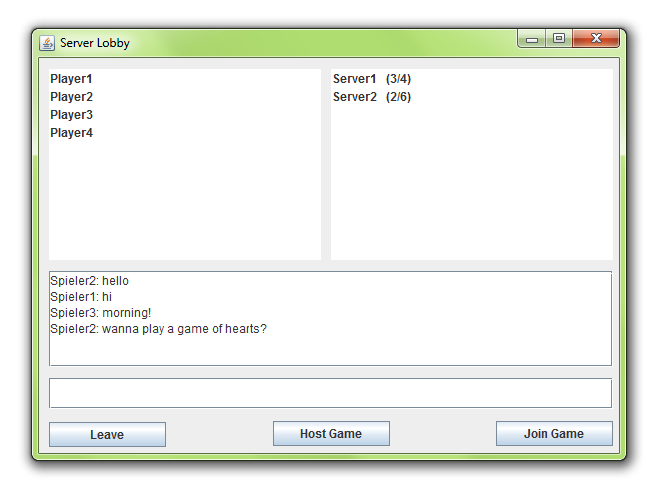
\includegraphics[scale=0.7]{GUI_images/ServerLobby}
	\item \gls{Erstellungsfenster}: \\ 
		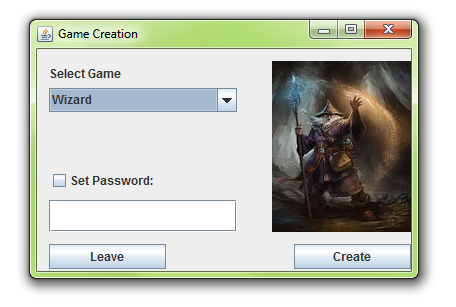
\includegraphics[scale=0.8]{GUI_images/CreateGame}
	\item \gls{Wartefenster}: \\ 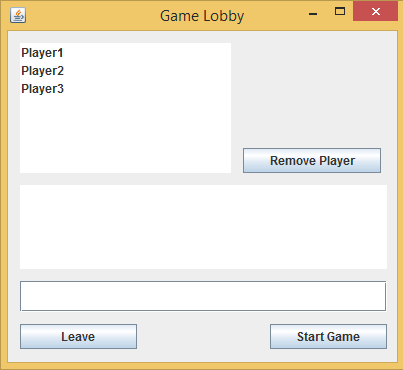
\includegraphics[scale=0.7]{GUI_images/GameLobby}
	\item Passwortabfrage: \\ 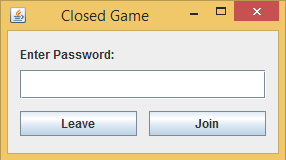
\includegraphics{GUI_images/PasswordRequest}
	\item Spiel: \\ 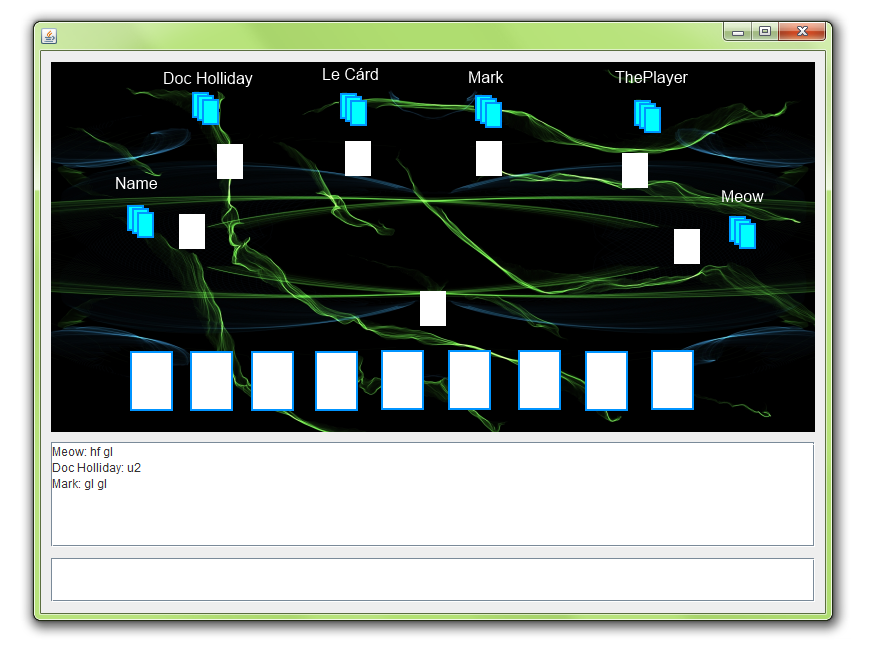
\includegraphics[scale=0.6]{GUI_images/GameClient}
\end{itemize}

\section{Testszenarien}
\begin{itemize}
	\item Startseite: \\ \\
		  Die folgenden Tests prüfen die Funktionalität der Startseite. \\
		  Für diese Tests werden keine Vorraussetzungen benötigt. \\
	\begin{itemize}
		\item Tests für /F045/. \\
			  Nach Eingabe von Benutzername und Serveradresse in /F040/. \\ \\
			  Eingabe einer korrekten Serveradresse und freiem Benutzernamen in /F040/
			  führt zum Verbindungsaufbau mit dem Server und anschließendem 
			  wechsel in die Server Lobby. \\ \\
			  Eingabe eines bereits verwendeten oder leeren Benutzernamens in /F040/
			  wird mit entsprechendem Hinweis quittiert. Die Startseite wird weiterhin angezeigt. \\ \\
			  Eingabe einer falschen Internetadresse in /F040/ wird mit entsprechendem Hinweis quittiert.
			  Die Startseite wird weiterhin angezeigt. \\ \\
		\item Test für /F050W/. \\ Im Dropdownmenü werden alle verfügbaren Sprachen angezeigt. \\ \\
			  Nach Auswahl einer Sprache wird die Startseite neu erstellt und alle darauf folgenden Fenster und 						  Dialoge in der ausgewählten Sprache angezeigt. 
			  
			  
	\end{itemize}

	\item Server Lobby: \\ \\
		  Die folgenden Tests prüfen die Funktionalität der Server Lobby. \\
		  Um die Tests auf dieser Ebene durchführen zu können ist eine aktive Serververbindung nach dem Login 					  erforderlich. \\
	\begin{itemize}
		\item Nach dem erscheinen der Server Lobby ist der zuvor gewählte Benutzername in /L30/ zu sehen. \\
			  Jeder weitere mit dem Server verbundene Client erscheint mit seinem eindeutigen Benutzernamen in /L30/.\\			  
		
		\item Tests für /F070/. \\
			  
	\end{itemize}
	
	\item Spiel erstellen (Lobby)
	\item Spiel beitreten (Lobby)
	\item Mehrere Spiele parallel starten (Lobby)
	\item Spiel spielen 
\end{itemize}

\section{Entwicklungsumgebung}
\subsection{Software}
\begin{itemize}
	\item LaTeX
	\item Eclipse
	\item IBM Rational Software Architect
	\item Git
\end{itemize}

\subsection{Hardware}
\begin{itemize}
	\item Rechner im CIP Pool	
	\item Private Rechner
\end{itemize}

\section{Ergaenzung}
..... 
\newpage
\printglossaries
\end{document}
